\proposedbox{
\section{Important technical documents published by MSL}

MSL can self-publish some types of document, such as our Technical Guide series and Callaghan Innovation technical reports. In doing so we should think about how to make these publications useful to others and consider to ensure they remain accessible. 

For example, links to important documents like our Technical Guides should continue working, even when the website appearance and content is updated. However, this is hard to achieve (who can take responsibility?). A better approach is to consider how to release documents that makes them resilient to change. 

This section considers how we can do that for our Technical Guides and Callaghan Innovation technical reports. 

\subsection{The FAIR principles}
The FAIR principles can be applied to enhance the value of digital assets, like our publications, in terms of use by others \cite{FAIR}. 

In relation to MSL publications, they can be interpreted as follows:
\begin{description}
	\item[Findable: ] A document must have a unique identifier (e.g., for searching and indexing purposes).  A Digital Object Identifier (DOI) is appropriate \cite{doi}. Several public science repositories issue a DOI when a document is deposited. Using one of these also takes care of the `A' principle, because the repository will also ensure that the document remains accessible.
	
	Authors should also be identified: each author should include their ORCID in the document \cite{orcid}.
	
	\item[Accessible: ] A document must be accessible (online). A distinction is made between knowing that a document exists (e.g., finding it in a search) and accessing it. 
	
	A document may still be protected from unauthorised use (e.g., by encryption) so openness is not implied.
	
	\item[Interoperable: ] A variety of applications should be able to use of the document. Publishing documents in PDF format (or better, in the PDF-A format) ensures that prospective readers have a choice of reading tools.
	  
	\item[Reusable: ] We publish documents for others to read, but sometimes also to reuse or re-distribute. Without a clear statement about copyright and licensing, a reader does not know if we give permission for the material to be reused. Permission should be explicitly granted, with an indication of acceptable ways of doing so. The Creative Commons licence, described in \S\ref{s_copyright}, is suitable. 

The provenance of work needs to be acknowledged too. Advice on how to cite (reference) a work should be included. 

\end{description}  

\subsection{Guidelines}
\subsection{Technical reports}
The figure below shows the appearance of an MSL technical report. Note the hyperlink to the DOI, where copies of the report are available. The green icon after the author's name is the orcid icon and is a hyperlink to orcid.

\begin{center}
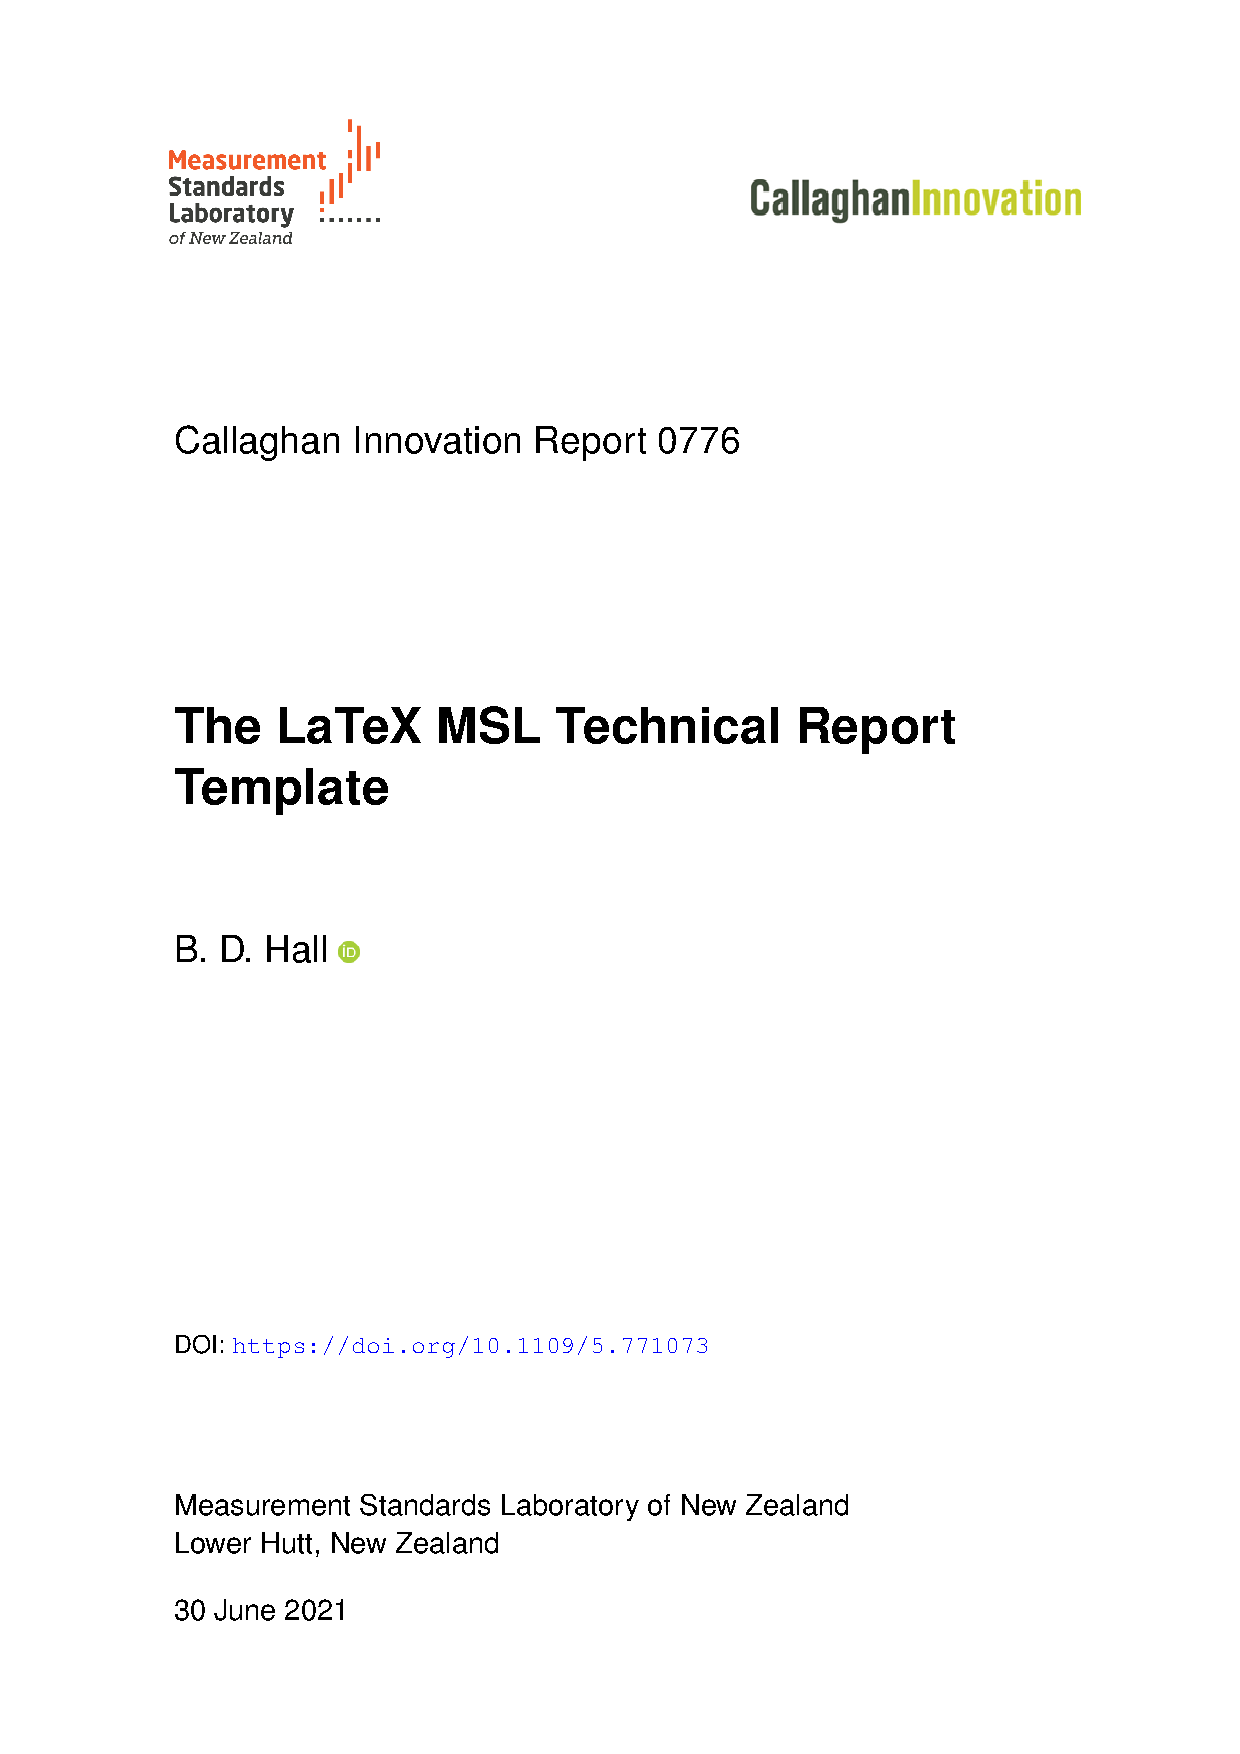
\includegraphics[scale=.5,page=1]{pictures/Report}
\end{center}

\newpage
The inside page of an MSL technical report repeats the title and includes a `reference', which suggests how the work can be cited, as shown below. The Creative-Commons licence is automatically placed after the summary / abstract material. 

\begin{center}
\includegraphics[scale=.5,page=2]{pictures/Report}
\end{center}

\subsection{Technical Guides}
The figure below shows the appearance of an MSL Technical Guide. The DOI is given in the header but not as a hyperlink.
\begin{center}
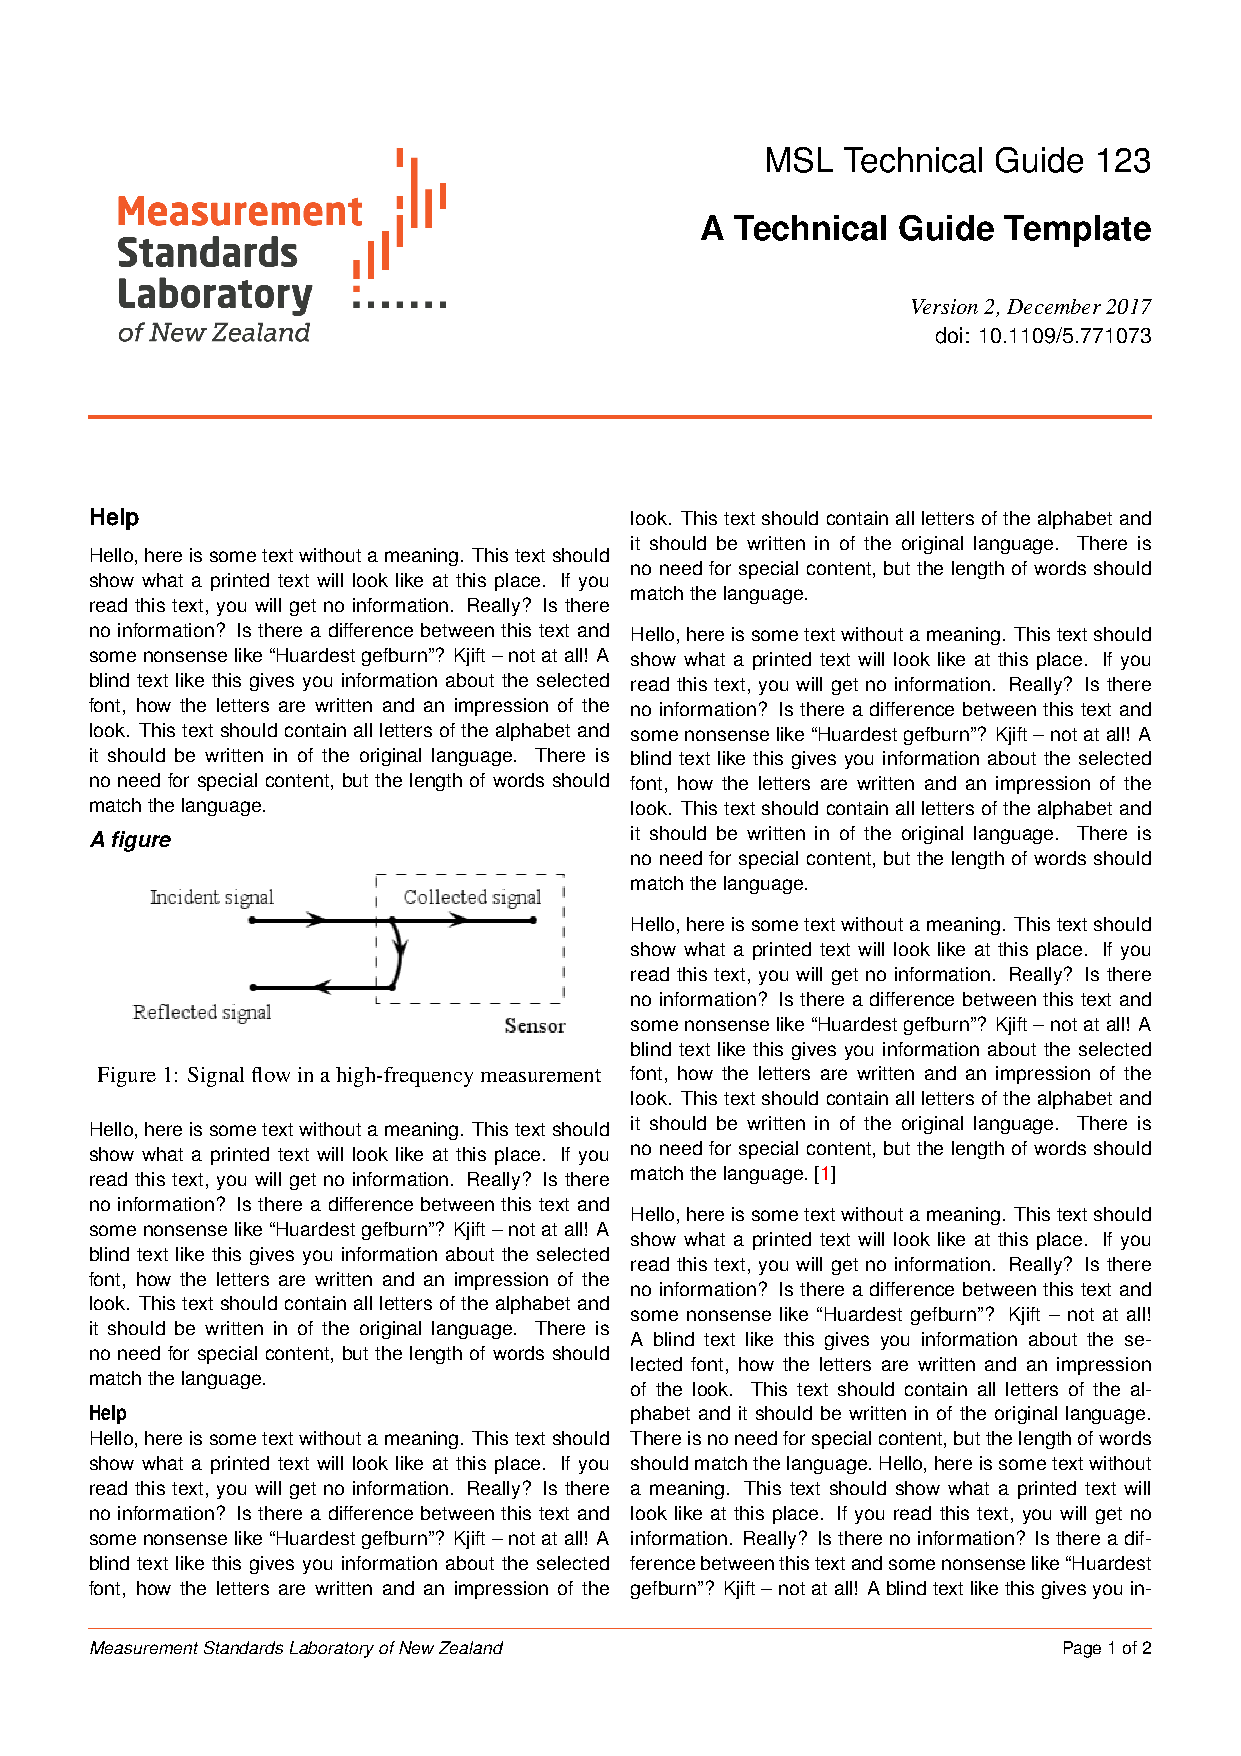
\includegraphics[scale=.5,page=1]{pictures/TG_Template}
\end{center}

\newpage
The last page of Technical Guide has an end-matter section where the names and orcids of the people who prepared the guide appear with other contact details. The doi is repeated here, but this time as a hyperlink. The Creative-Commons licence is automatically included.

\begin{center}
\includegraphics[scale=.5,page=2]{pictures/TG_Template}
\end{center}
}%